%!TEX root = /Users/louis/Documents/PhD/Deliverables/Thesis/thesis.tex

\section{Metamodel-Independent Syntax}
\label{sec:mmi_syntax}
Section~\ref{subsec:modelling_framework_characteristics} discussed the way in which modelling frameworks implicitly enforce conformance, and hence prevent the loading of non-conformant models. Additionally, modelling frameworks provide little support for checking the conformance of a model with other versions of a metamodel, which is potentially useful during metamodel installation. In Section~\ref{sec:requirements_identification}, these concerns lead to the identification of the following requirement: \emph{This thesis must investigate the extension of existing modelling frameworks to support the loading of non-conformant models and conformance checking of models against other metamodels.}

This section describes the way in which existing modelling frameworks load and store models using a metamodel-specific binding mechanisms, proposes an alternative binding mechanism using a metamodel-independent representation, and demonstrates how this facilitates automatic consistency checking. The work presented in this section has been published in \cite{rose09enhanced}.

% TODO - present MM independent syntax. Make clear that it is an ABSTRACT syntax.

\begin{figure}[htbp]
	\centering
	\subfigure[Original metamodel.]
	{
	    \label{fig:original_families_mm}
	    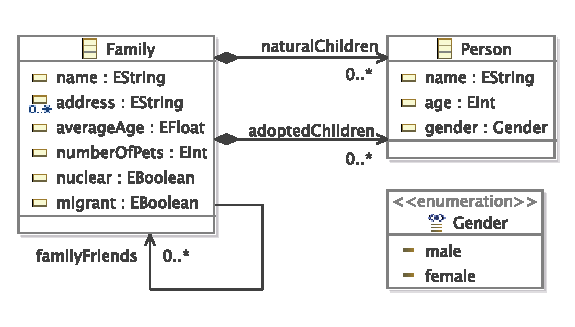
\includegraphics[scale=0.9]{5.Implementation/images/families.pdf}
	}
	\subfigure[Evolved metamodel.]
	{
	    \label{fig:evolved_families_mm}
	    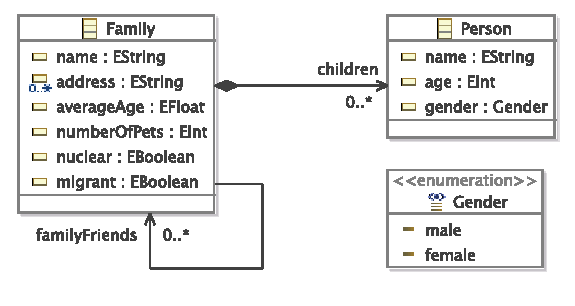
\includegraphics[scale=0.9]{5.Implementation/images/families_evolved.pdf}
	}
	\caption{Evolution of a families metamodel.}
\label{fig:families_mms}
\end{figure}

\subsection{Metamodel Evolution Example: Families}
\label{subsec:families_example}
This section uses the example of metamodel evolution in Figure~\ref{fig:families_mms}, which illustrates changes to a metamodel for describing families. In Figure~\ref{fig:original_families_mm}, \texttt{na\-tu\-r\-alCh\-il\-dr\-en} and \texttt{ad\-op\-t\-edCh\-il\-dr\-en} are modelled as separate features, and, in Figure~\ref{fig:evolved_families_mm}, they are modelled as a single feature, \texttt{ch\-il\-dr\-en}.

A model that conforms to the original metamodel, such as the one in Figure~\ref{fig:families_model},  might not conform to the evolved metamodel. Specifically, models that specify values for the \texttt{na\-tu\-r\-alCh\-il\-dr\-en} or \texttt{ad\-op\-t\-edCh\-il\-dr\-en} features do not conform to the evolved metamodel. The model in Figure~\ref{fig:families_model} represents a \texttt{Fa\-mi\-ly} comprising two \texttt{Pe\-rs\-on}s, and does not conform to the evolved metamodel. Using the families metamodel and model, the sequel explains why existing modelling frameworks cannot be used to load non-conformant models.

\begin{figure}[htbp]
  \begin{center}
    \leavevmode
    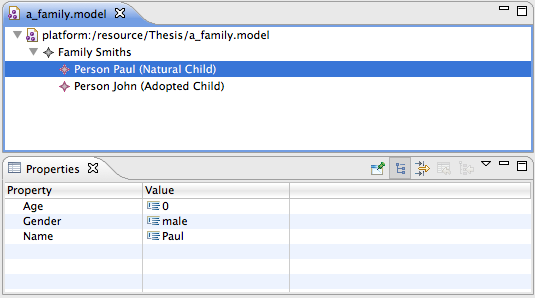
\includegraphics[width=10cm]{5.Implementation/images/family_model.png}
  \end{center}
  \caption[A family model]{A family model, conforming to Figure~\ref{fig:original_families_mm}}
  \label{fig:families_model}
\end{figure}


\subsection{Binding to a Specific Metamodel}
\label{subsec:binding_specific}
To load a model, existing modelling frameworks construct objects in the underlying programming language in a process termed \emph{binding} (Section~\ref{subsec:modelling_framework_characteristics}). The metamodel defines the way in which model elements will be bound, and binding is strongly-typed. Figure~\ref{fig:successful_binding} illustrates the results of binding the family model in Figure~\ref{fig:families_model} to the original families metamodel in Figure~\ref{fig:original_families_mm}. The objects in Figure~\ref{fig:successful_binding} instantiate types that are defined in the metamodel, such as \texttt{Fa\-mi\-ly} and \texttt{Pe\-rs\-on}. In other words, binding results in a \emph{metamodel-specific} representation of the model.

\begin{figure}[htbp]
  \centering
  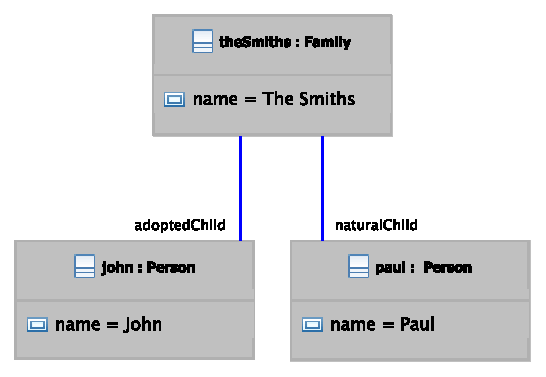
\includegraphics[height=5cm]{5.Implementation/images/successful_binding.pdf}
  \caption{Objects resulting from the binding of a conformant model}
  \label{fig:successful_binding}
\end{figure}

Metamodel-specific binding fails for non-conformant models. For example, attempting to bind the family model in Figure~\ref{fig:families_model} to the evolved families fails because the model uses \texttt{na\-tu\-r\-alCh\-il\-dr\-en} and \texttt{ad\-op\-t\-edCh\-il\-dr\-en} features for the type \texttt{Fa\-mi\-ly}, and these features are not defined by the metamodel in Figure~\ref{fig:evolved_families_mm}.

Because non-conformant models cannot be loaded, model migration must be performed by editing the underlying storage representation, which can be error-prone and tedious (Section~\ref{subsec:user-driven_co-evolution}). The sequel discusses potential solutions for loading non-conformant models.

\subsection{Potential Solutions for Loading Non-Conformant Models}
Two potential approaches to binding (and hence loading) non-conformant models have been considered and are now discussed. The benefits and drawbacks of each approach have been compared, which resulted in the selection of the second approach, binding to a metamodel-independent syntax.

\subsubsection{Store metamodel history}
Presently, modelling frameworks are used to store only the latest version of a metamodel, and hence binding fails for models that conform to a previous version of the metamodel. If modelling frameworks could access old versions of a metamodel, models that do not conform to the current version of the metamodel could be loaded by binding to a previous version of the metamodel.

\subsubsection{A metamodel-independent syntax}
Binding to a metamodel-specific representation fails for non-conformant models. An alternative, therefore, is to bind models to a \emph{metamodel-independent} representation in the underlying programming language, such as the one shown in Figure~\ref{fig:minimal_generic_metamodel}. Binding each model element would result in the instantiation of a metamodel-independent type (\texttt{Ob\-je\-ct} in Figure~\ref{fig:minimal_generic_metamodel}) rather than of types defined in the metamodel, such as \texttt{Fa\-mi\-ly} or \texttt{Pe\-rs\-on}. Therefore binding is independent of the types defined in metamodels, and will succeed for non-conformant models.

\begin{figure}[htbp]
  \centering
  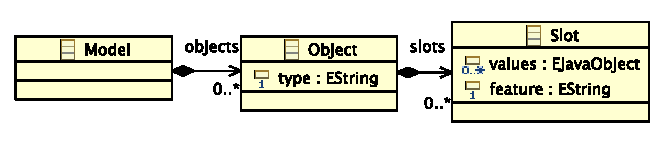
\includegraphics[width=3.3in]{5.Implementation/slot_model.pdf}
  \caption[A minimal generic metamodel for MOF]{A minimal generic metamodel for MOF, based on \cite{mof} and taken from \cite{rose09enhanced}.}
  \label{fig:minimal_generic_metamodel}
\end{figure}
   
\subsubsection{Benefits and drawbacks of the potential solutions}
The two potential solutions for loading non-conformant models have different benefits and drawbacks, which are now discussed. Storing metamodel histories would use the binding and conformance checking services provided by existing modelling frameworks, and therefore require less implementation effort than a metamodel-independent syntax, which would use require bespoke binding and conformance checking services. Furthermore, structures for managing metamodel histories might be integrated with existing approaches to managing co-evolution, such as metamodel differencing approaches (Sections~\ref{subsec:inference}), for switching between different versions of a MDE workflow.

Storing metamodel histories relies on the metamodel developer to enable model migration: if the metamodel developer does not provide a metamodel that contains historical data, then binding will fail for non-conformant models. Conversely, models can be bound to a metamodel-independent syntax irrespective of the actions of the metamodel developer.

A metamodel-independent syntax has been chosen because it makes fewer assumptions of the metamodel developer, and hence facilitates user-driven as well as developer-driven co-evolution.


\subsection{Proposed Solution: A Metamodel-Independent Syntax}
\label{subsec:binding}
This section discusses the design and implementation of a metamodel-independent syntax, and of the binding and conformance checking services that are used to load non-conformant models. As discussed below, the design of the metamodel-independent syntax and conformance checking service is inspired by \cite{uml212} and \cite{paige07metamodel}, respectively. As such, the primary contribution of this section is the implementation and integration of the syntax and services with EMF, which is described in Section~\ref{subsubsec:mmi_impl}. Additionally, the syntax and services have been designed to be re-usable, and hence have been used to simplify the implementation of a textual modelling notation (Section~\ref{sec:notation}) and a model migration language (Section~\ref{sec:flock}).

\subsubsection{Design}
A high-level design for the way in which the metamodel-independent syntax, binding service and conformance checking service load models is shown in Figure~\ref{fig:mmi_workflow}. The \textbf{binding service} parses XMI (the canonical storage representation of models, Section~\ref{subsec:mof}) and produces a set of objects that conform to the \textbf{metamodel-independent syntax}. The \textbf{conformance checking service} is used to explicitly check the conformance of a bound model represented in the metamodel-independent syntax.

Binding and conformance checking were split into separate services to facilitate re-use. For example, the textual modelling notation in Section~\ref{sec:notation} re-uses the metamodel-independent syntax and conformance checking service, in conjunction with a different binding service.

\paragraph{Metamodel-independent syntax} The metamodel-independent syntax is used to represent a model without instantiating types defined by its metamodel. Its design was inspired by the metamodel for UML 2 \cite{uml212} object diagram, which describes objects in a generic, class-independent manner. UML 2 object diagrams are specified in terms of an abstract syntax (comprising, for example, \texttt{InstanceSpecification} and \texttt{Link} classes) and a concrete syntax (comprising, for example, boxes and lines). The metamodel-independent syntax proposed here is abstract. It is not used directly by metamodel developers or users and hence a concrete syntax was not required.

Abstract syntax is typically represented as a metamodel (Section~\ref{subsec:modelling_languages}), and the metamodel that was designed for the metamodel-independent syntax is shown in Figure~\ref{fig:mmi_syntax_design}. \texttt{Ob\-je\-ct}s are used to represent each element of a model, and the \texttt{ty\-pe} attribute is used to indicate the name of the metaclass that the \texttt{Ob\-je\-ct} intends to instantiate. Similarly, \texttt{Sl\-ot}s are used to represent values in the model, and the \texttt{feature} attribute indicates the metafeature to which the value belongs. The metamodel was designed to capture the information needed to perform conformance checking (described below), and implementing the conformance checking service led to a refactored metamodel, which is presented in the sequel.

% TODO - show complete MMI syntax, with model elements

COPE (Section~\ref{sec:subsec:operator-based_co-evolution}) is also built atop a metamodel-independent syntax. However, the metamodel-independent syntaxes used by COPE and proposed here were developed independently, and both were first published in 2008 (in \cite{rose08hutn,herrmannsdoerfer08cope}).

\paragraph{Metamodel-independent binding service} Binding a textual representation of a model to a metamodel is a model-to-text (M2T) transformation. The metamodel-independent binding service is a M2T transformation that consumes XMI and produces a model conforming to the metamodel-independent syntax. The transformation iterates over each tag in the XMI, and creates instances of \texttt{Ob\-je\-ct} and \texttt{Sl\-ot}. For example, when encountering a tag that represent a model element, the transformation:

\begin{enumerate}
	\item Constructs an instance of \texttt{Ob\-je\-ct}, \texttt{o}.
	\item For each attribute of the tag:
	\subitem Creates an instance of \texttt{Sl\-ot}, \texttt{s}.
	\subitem Sets \texttt{s.feature} to the name of the attribute.
	\subitem Sets \texttt{s.value} to the value of the attribute.
	\subitem Adds \texttt{s} to \texttt{o.slots}.
	\item For each child tag:
	\subitem Creates an instance of \texttt{Sl\-ot}, \texttt{s}.
	\subitem Sets \texttt{s.feature} to the name of the child tag.
	\subitem Recursively constructs an instance of \texttt{Ob\-je\-ct}, c.
	\subitem Sets \texttt{s.value} to c.
	\subitem Adds \texttt{s} to \texttt{o.slots}.
\end{enumerate}


\paragraph{Conformance checking service} Conformance is a type of inter-model consistency, between a model and its metamodel (Section~\ref{subsec:modelling_languages}), and, in MDE, inter-model consistency is often validated using a set of constraints (Section~\ref{subsubsec:model_validation}). Furthermore, \cite{paige07metamodel} demonstrates that conformance can be specified as a set of constraints between a model and its metamodel. As such, the conformance checking service has been designed as the set of constraints between models and metamodels in Figure~\ref{fig:conformance_checking_constraints}.

The conformance checking service must be interoperable with the metamodel-independent syntax and, hence, the constraints are specified in terms of \texttt{Ob\-je\-ct}s and \texttt{Sl\-ot}s. Clearly, to check conformance the constraints must refer to a (specific) metamodel, and the constraints are also specified in terms of concepts from the MOF metamodelling language (Section~\ref{subsec:mof}), such as \texttt{Class} and \texttt{Property}. Figure~\ref{fig:minimal_mof} shows a minimal version of the MOF metamodel.

% TODO - show minimal MOF metamodel that is consistent with the following constraints

\begin{figure}[htbp]
	\begin{framed}
	  \begin{enumerate}
			\item Each \texttt{Ob\-je\-ct}'s \texttt{ty\-pe} must be the \texttt{na\-me} of some non-\texttt{ab\-str\-act} metamodel \texttt{Cl\-a\-ss}.
			\item Each \texttt{Ob\-je\-ct} must specify a \texttt{Sl\-ot} for each mandatory \texttt{Pr\-op\-er\-ty} of its \texttt{ty\-pe}.
			\item Each \texttt{Sl\-ot}'s \texttt{fe\-at\-u\-re} must be the name of a metamodel \texttt{Pr\-op\-er\-ty}. That \texttt{Pr\-op\-er\-ty} must belong to the \texttt{Sl\-ot}'s \texttt{ow\-n\-er}'s \texttt{ty\-pe}.
			\item Each \texttt{Sl\-ot} must be multiplicity-compatible with its \texttt{Pr\-op\-er\-ty}. More specifically, each \texttt{Sl\-ot} must contain at least as many values as its \texttt{Pr\-op\-er\-ty}'s \texttt{lo\-w\-er} bound, and at most as many values as its \texttt{Pr\-op\-er\-ty}'s \texttt{up\-p\-er} bound.
		  \item Each \texttt{Sl\-ot} must be type-compatible with its \texttt{Pr\-op\-er\-ty}. (The way in which type-compatibility is checked depends on the way in which the modelling framework is implemented).
		\end{enumerate}
	\end{framed}
  \caption{The constraints of the conformance checking service.}
  \label{fig:minimal_generic_metamodel}
\end{figure}


\subsubsection{Reference implementation in Java, EMF and Epsilon}
\label{subsubsec:mmi_impl}
Reference implementations of the three components were constructed with Java, EMF and Epsilon (Section~\ref{sec:mde_tools}). The way in which each component was implemented is now discussed.

\paragraph{Metamodel-independent syntax} Ecore, the metamodelling language of EMF, was used to implement the metamodel-independent syntax. The final metamodel is shown in Figure~\ref{fig:mmi_in_ecore}, which differs slightly to the design discussed above. Specifically, only one feature refers directly to the metamodel, which simplifies the construction of models conforming to the metamodel. The references between \texttt{Cl\-a\-ssOb\-je\-ct} and \texttt{ECl\-a\-ss} and Slot and \texttt{ESt\-ru\-ct\-ur\-alFe\-at\-u\-re} are implemented as derived features (i.e. they are computed at runtime, using the \texttt{me\-ta\-mo\-del} reference). 

\paragraph{Binding service} A text-to-model (T2M) transformation language (Section~\ref{subsubsec:model_transformation}) could have been used to implement the binding service. However, in 2008 the Eclipse Modeling Project\footnote{\url{http://www.eclipse.org/modeling/}} did not provide a standard T2M language and using a T2M language that was not part of the Eclipse Modeling Project would have complicated installation of the service for users.

Instead, the binding service has been implemented by constructing in Java an XMI parser that emits objects conforming to the metamodel-independent syntax. Listing~\ref{lst:xmi_parser} illustrates the way in which XMI attributes are parsed. The \texttt{pr\-oc\-e\-ssAtt\-rib\-ut\-es} method is called to generate instances of \texttt{At\-tr\-ibu\-teSl\-ot} from the metamodel-independent syntax. For each attribute in an XMI tag, the body of the loop is executed. If the attribute is not XMI metadata such as type information (line 4), the name and value of the attribute (lines 5 and 6) are extracted from the XMI, and used to add the value to an \texttt{At\-tr\-ibu\-teSl\-ot} with feature equal to the name of the attribute (line 8). Constructing \texttt{O\-bj\-e\-ct}s and \texttt{Sl\-ot}s is the responsibility of the \texttt{ge\-ne\-ra\-tor} object, which is an instance variable of the parser.


\begin{lstlisting}[caption=Parsing XMI attributes (in Java), label=lst:xmi_parser, language=Java]
private void processAttributes(Attributes atts) {
	for (int index = 0; index < atts.getLength(); index++) {
		
		if (!attributeIsMetadata(atts.getQName(index))) {
			final String feature = atts.getLocalName(index);
			final String value   = atts.getValue(index);
			
			generator.addAttributeValue(feature, value, getCurrentLineNumber());
		}
	}
}
\end{lstlisting}

\paragraph{Conformance checking service} The conformance constraints were specified in EVL \cite{kolovos08evl}, a language tailored to specifying model verification, and hence suitable for rapid prototyping of consistency constraints. Listing~\ref{lst:conformance_constraint} shows the EVL that checks that each \texttt{ClassObject}'s type is a non-abstract class (constraint 1, above). The check part (line 3) verifies that a particular \texttt{ClassObject} (\texttt{self}) refers to a metamodel type that is not abstract. When the check fails, the message (line 4) is automatically added to a set of unsatisfied constraints by EVL. The \texttt{toClass} operation (lines 8-10) is used to determine the metamodel class (an instance of \texttt{EClass}) to which the \texttt{type} attribute (a String) of a \texttt{ClassObject} refers.

\begin{lstlisting}[caption=A constraint (in EVL) to check that only concrete metamodel types are instantiated., label=lst:conformance_constraint, language=EVL]
context ClassObject {
	constraint ClassMustNotBeAbstract {
		check: not self.toClass().isAbstract()
		message: 'Cannot instantiate the abstract class: ' + self.type
	}
}

operation ClassObject toClass() : EClass {
	return Metamodel!EClass.all.selectOne(c|c.name == self.type);
}
\end{lstlisting}

Type-compatibility has been implemented by delegating to the type-checking methods provided by EMF. The EVL constraints call methods on the \texttt{Slot} class (defined in the metamodel-independent syntax), which in turn call methods defined by EMF.
% TODO - resinstate this?
% In EMF, for example, model values conform either to types defined in a metamodel, or to types defined in the underlying programming language, Java. The sequel describes the way in type-compatibility checking has been implemented for the conformance checking service.
		%Conformance constraints vary over modelling languages. For example, Ecore, the modelling language of EMF, is similar to but not the same as MOF. Metamodel features defined in Ecore can be marked as transient (not stored to disk) or unchangeable (read-only). Consequently in EMF, conformance constraints are required to restrict the feature value of slots to only non-transient, changeable features.

\subsubsection{An example of binding to a metamodel-independent syntax}
\label{subsec:mmi_syntax_example}
The example in Section~\ref{subsec:families_example} is re-visited to demonstrate the way in which a metamodel-independent syntax can be used to load a non-conformant model. Binding the model in Figure~\ref{fig:families_model} to the metamodel-independent syntax shown in Figure~\ref{fig:slot_model} produces three instances of \texttt{Ob\-je\-ct}, illustrated as a UML object diagram in Figure~\ref{fig:generic_binding}. For clarity, instances of \texttt{Ob\-je\-ct} are shaded, and instances of \texttt{Sl\-ot} are unshaded. The first \texttt{Ob\-je\-ct} represents the \texttt{Fa\-mi\-ly} model element and has three slots. Two of the slots are used to reference the \texttt{Pe\-rs\-on} model elements via the \texttt{na\-tu\-r\-alCh\-il\-dr\-en} and \texttt{ad\-op\-t\-edCh\-il\-dr\-en} references. When binding to a generic metamodel, models are represented in terms of a set of types that is metamodel-independent (\texttt{Mo\-d\-el}, \texttt{Ob\-je\-ct} and \texttt{Sl\-ot}), and hence binding succeeds for conformant and non-conformant models.

\begin{figure}[htbp]
  \centering
  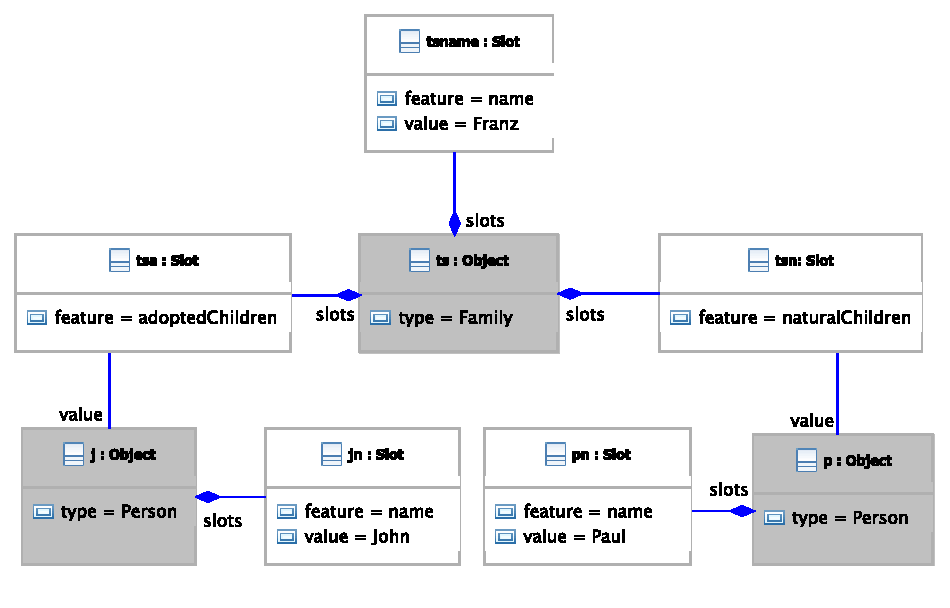
\includegraphics[width=12cm]{5.Implementation/images/generic_binding.pdf}
  \caption{Exemplar instantiation of generic metamodel.}
  \label{fig:generic_binding}
\end{figure}

After binding to the metamodel-independent syntax, the conformance of a model can be checked against any specific metamodel. To illustrate the value of the generic metamodel, consider again the metamodel evolution in Figure~\ref{fig:original_families_mm} and the model in Figure~\ref{fig:evolved_families_mm}. Conformance checking for the model element representing the \texttt{Fa\-mi\-ly} would now fail because it defines slots for features named  \texttt{na\-tu\-r\-alCh\-il\-dr\-en} and \texttt{ad\-op\-t\-edCh\-il\-dr\-en}, which are no longer defined for the metamodel class \texttt{Fa\-mi\-ly}. Specifically, the model element representing the \texttt{Fa\-mi\-ly} does not satisfy conformance constraint 4 (Section~\ref{subsec:binding}), which states: \emph{each slot's feature must be the name of a metamodel feature. That metamodel feature must belong to the slot's owning object's type}. 

\subsection{Structures built atop the metamodel-independent syntax}
There are many potential uses for the components described in this section. Section~\ref{sec:notation} describes a textual modelling notation integrated with the metamodel-independent syntax to achieve live conformance checking. The migration language presented in Section~\ref{sec:flock} can be used with the metamodel independent syntax to perform partial migration (i.e. to produce models that conform to a generic metamodel rather than their evolved metamodel), but implementation of this work is not complete\footnote{The current version does not support partial migration of non-containment references and enumeration types.}.

In addition to these uses, the metamodel-independent syntax is potentially useful during metamodel installation. As discussed in Section~\ref{subsec:modelling_framework_characteristics}, metamodel developers do not have access to downstream models, and conformance is implicitly enforced by modelling frameworks. Consequently, the conformance of models may be affected by the installation of a new version of a metamodel, and the conformance of models cannot be checked during installation. Typically, installing a new version of a metamodel can result in models that no longer conform to their metamodel and cannot be used with the modelling framework. Moreover, a user discovers conformance problems only when attempting to use a model after installation has completed, and not as part of the installation process.

% TODO - Consider discussing the number of revisions of say, UML (and other metamodels), in Chapter 2. This will allow the reader to get a sense of the scale of the problem.

To enable conformance checking as part of metamodel installation in EMF, the metamodel-independent syntax has been integrated with Concordance in \cite{rose10concordance}. The work was conducted outside of the scope of the thesis, and is now summarised to indicate the usefulness of the metamodel-independent syntax for supporting the automation of co-evolution activities. Concordance provides a mechanism for resolving inter-model references (such as those between models and their metamodels). Without Concordance, determining the the instances of a metamodel is possible only by checking every model in the workspace. Integrating Concordance and the metamodel-independent syntax resulted in a service, which Epsilon (Section~\ref{subsec:epsilon}) executes after the installation of a metamodel to identify the models that are affected by the metamodel changes. All models that conform to the old version of the metamodel are checked for conformance with the new metamodel. As such, conformance checking occurs automatically and immediately after metamodel installation. Conformance problems are detected and reported immediately, rather than when an affected model is next used.

\subsubsection{Summary}
Modelling frameworks implicitly enforce conformance, which presents challenges for managing co-evolution. In particular, detecting and reconciling conformance problems involves managing non-conformant models, which cannot be loaded by modelling frameworks and hence cannot be used with model editors or model management operations. The metamodel-independent syntax proposed in this section enables modelling frameworks to load non-conformant models by binding models to a generic metamodel. The metamodel-independent syntax has been integrated with Concordance \cite{rose10concordance} to facilitate the reporting of conformance problems during metamodel installation, and underpins the implementation of the textual modelling notation presented in Sections~\ref{sec:notation}. The benefits and drawbacks of the metamodel-independent syntax in the context of user-driven co-evolution are explored in Chapter~\ref{Evaluation}. 
